\section{Theorie}

\subsection{Kathodenstrahlröhre}

Die Erzeugung eines Elektronenstrahls kann mit einer
Kathodenstrahlröhre durchgeführt werden. Der schematische Aufbau dieser ist in
Abbildung \ref{abb:1} dargestellt. Die Kathodenstrahlröhre ist evakuiert, da sonst
die Elektronen mit den Luftmolekülen Wechselwirken würden.

\begin{figure}[H]
  \centering
  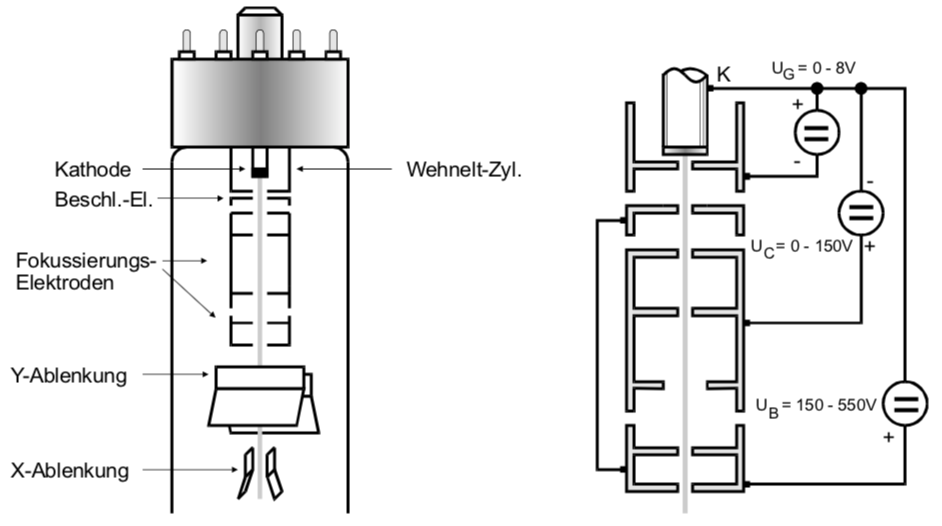
\includegraphics[width=\textwidth]{content/Kathode.png}
  \caption{Schematische Darstellung einer Kathodenstrahlröhre \cite{1}.}
  \label{abb:1}
\end{figure}

Die Kathodenstrahlröhre besteht aus drei Teilen.
Im ersten Teil werden die Elektronen durch Glühemission einer Kathode erzeugt.
Diese Kathode ist von einem Wehnelt-Zylinder umgeben, an dem eine Gegenspannung
der Kathode gegenüber anliegt. Durch diese Spannung kann die Intensität des Elektronenstrahls
eingestellt werden. Daraufhin folgt eine starke Beschleunigungsspannung $U_B$. Während
der Beschleunigung wird der Elektronenstrahl durch inhomogene elektrische Felder fokussiert.
Die Geschwindigkeit $v_z$, auf welche die Elektronen beschleunigt werden lässt sich aus dem
Energiesatz

\begin{equation}
  \frac{m_0 v_z^2}{2} = e_0 U_b
  \label{lala}
\end{equation}
herleiten.

Dabei ist $m_0$ die Elektronenmasse und $e_0$ die Elementarladung.

In dem zweiten Teil befindet sich das Ablenksystem für den Elektronenstrahl. Dieses
besteht aus zwei senkrecht zueinander stehenden Kondensatoren. Damit kann der Elektronenstrahl
in zwei Richtungen abgelenkt werden.
Als letztes folgt ein Leuchtschirm, der an dem Auftreffpunkt des Elektronenstrahls
leuchtet.
\subsection{Ablenkung im elektrischen Feld}
Nun wird ein Zusammenhang zwischen der Verschiebung $D$ auf dem Schirm und der
Ablenkspannung $U_d$ hergeleitet. Dazu werden die in Abbildung \ref{abb:2} angegebenen
Bezeichnungen verwendet.

\begin{figure}[H]
  \centering
  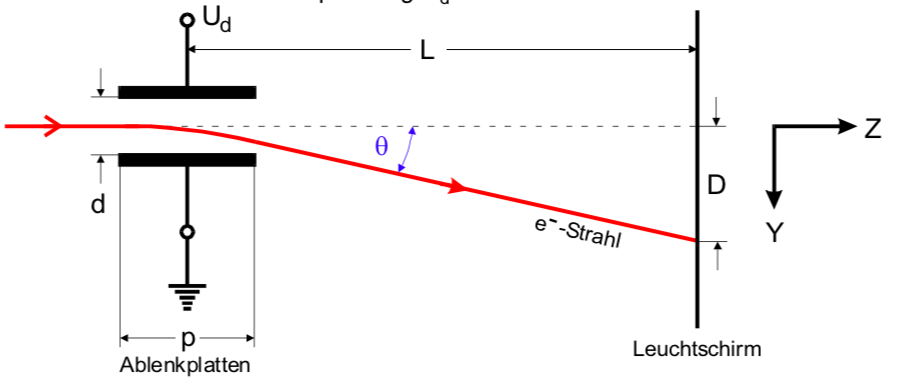
\includegraphics[width=\textwidth]{content/Ablenkung.png}
  \caption{Skizze des Ablenkvorganges in einer Kathodenstrahlröhre \cite{1}.}
  \label{abb:2}
\end{figure}

Mithilfe geometrischer Überlegungen und Energiesatz \ref{lala} folgt dann der Zusammenhang

\begin{equation}
  D = \frac{p}{2d} L \frac{U_d}{U_B}.
  \label{eq:1}
\end{equation}

Mit einer Kathodenstrahlröhre kann außerdem ein Oszillograph realisiert werden,
der eine Zeitabhängige Wechselspannung darstellen kann. Dazu wird an das Plattenpaar,
welches für die horizontale Ablenkung verantwortlich ist, eine Sägezahnspannung angeschlossen.
Diese steigt mit der Zeit an und springt bei einem Maximalwert wieder auf den Anfangswert
zurück. An das andere Plattenpaar wird dann die zu untersuchende Wechselspannung angeschlossen.
Damit stehende Wellen auf dem Leuchtschirm dargestellt werden können müssen die
Frequenzen der beiden Spannungen die Synchronisationsbedingung erfüllen:

\begin{equation}
  n \nu_\text{Sä} = m \nu_\text{We} \,\,\,\,\, \text{mit} \, \, \, n=1, 2, 3, ... \, \, \, m=1, 2, 3, ...
  \label{eq:2}
\end{equation}


\subsection{Elektronenstrahl im transversalen Magnetfeld}

Auf eine Ladung $q$ in homogenen Magnetfeldern $\vec{B}$ wirkt die Lorentz-Kraft

\begin{equation*}
  \vec{F_L} = q \vec{v} \times \vec{B}.
\end{equation*}

Dabei ist $\vec{v}$ die Geschwindigkeit der Ladung. Ein Magnetfeld lenkt eine Ladung
also ab, allerdings wird an der Ladung keine Arbeit verrichtet. Das bedeutet, dass
$|\vec{v}|$ konstant bleibt und somit bewegt sich die Ladung auf einer Kreisbahn im Magnetfeld,
wenn sie senkrecht in das Magnetfeld eindringt.

In Abbildung \ref{bild:1} ist der Ablenkvorgang eines Elektronenstrahls in einem
Magnetfeld gezeigt.

\begin{figure}[H]
  \centering
  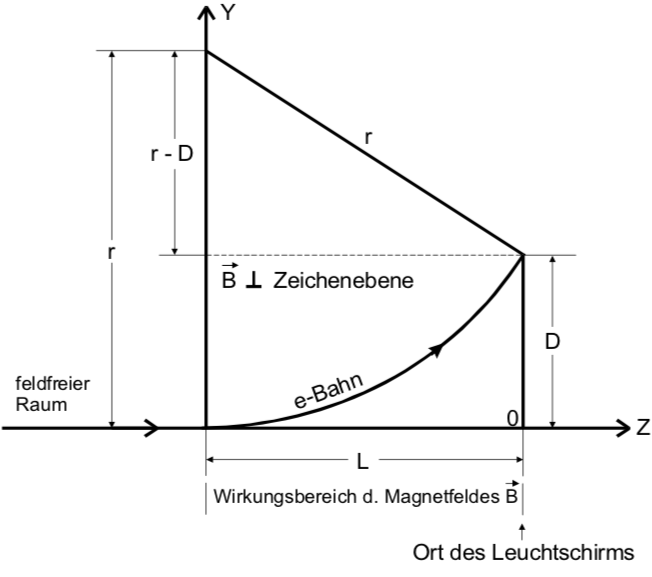
\includegraphics[width=\textwidth]{content/B-Feld.png}
  \caption{Schematische Darstellung des Ablenkvorganges im B-Feld \cite{2}.}
  \label{bild:1}
\end{figure}



Mithilfe einer Kathodenstrahlröhre und einem homogenen Magnetfeld lässt sich nun
die spezifische Ladung von Elektronen $\frac{e_0}{m_0}$ bestimmen.
Zur Herleitung einer Gleichung für $\frac{e_0}{m_0}$, wird der Satz des Pythagoras
auf die in Abbildung \ref{bild:1} gezeigten Beziehungen zwischen $D$, $L$ und $r$ angewendet.
Der Zusammenhang zwischen Ablenkung $D$ und spezifische Ladung der Elektronen ergibt sich somit zu

\begin{equation}
  \frac{D}{L^2 + D^2} = \frac{1}{\sqrt{8 U_B}} \sqrt{\frac{e_0}{m_0}} B.
  \label{eq:3}
\end{equation}

\newpage

Auf der Erde gibt es das \enquote{Erdmagnetfeld}, welches die Erde durchdringt und umgibt.
Dieses Erdmagnetfeld hat ungefähr die Form von dem Feld eines magnetischen Dipols. Dabei ist die
Dipolachse leicht verschoben von der Erdachse.
Wird auf der Oberfläche der Erde das Erdmagnetfeld lokal gemessen, so wird nur die horizontale Komponente des
Magnetfeldes gemessen. Um aus der horizontalen Komponente nun das gesamte Magnetfeld zu errechnen
wird der sogenannte \enquote{Inklinationswinkel} verwendet. Der Inklinationswinkel
ist der Winkel zwischen der Horizontalebene, also die Ebene in der das Erdmagnetfeld gemessen wird,
und der tatsächlichen Richtung des Erdmagnetfeldes.
